\begin{figure}[t]
	\centering
	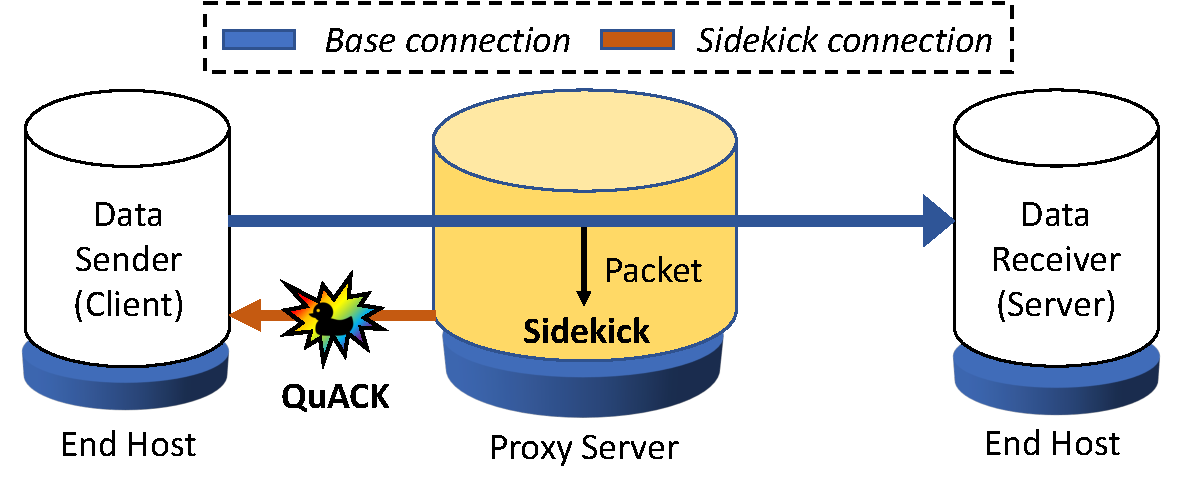
\includegraphics[width=\linewidth]{sidekick-paper/figures/sc_protocol.pdf}
\caption{The proxy generates quACKs, in-network acknowledgments, based on
the opaque packets it observes in the base protocol. It quACKs to an end
host, the data sender, which sends or resends packets on the base protocol as a result.
Although we only show one side of the connection, the Sidekick could assist
either end host of a bidirectional flow.
}
\label{fig:sc-protocols}
\end{figure}
